\begin{figure*}
\begin{center}

\begin{subfigure}[b]{\columnwidth}
  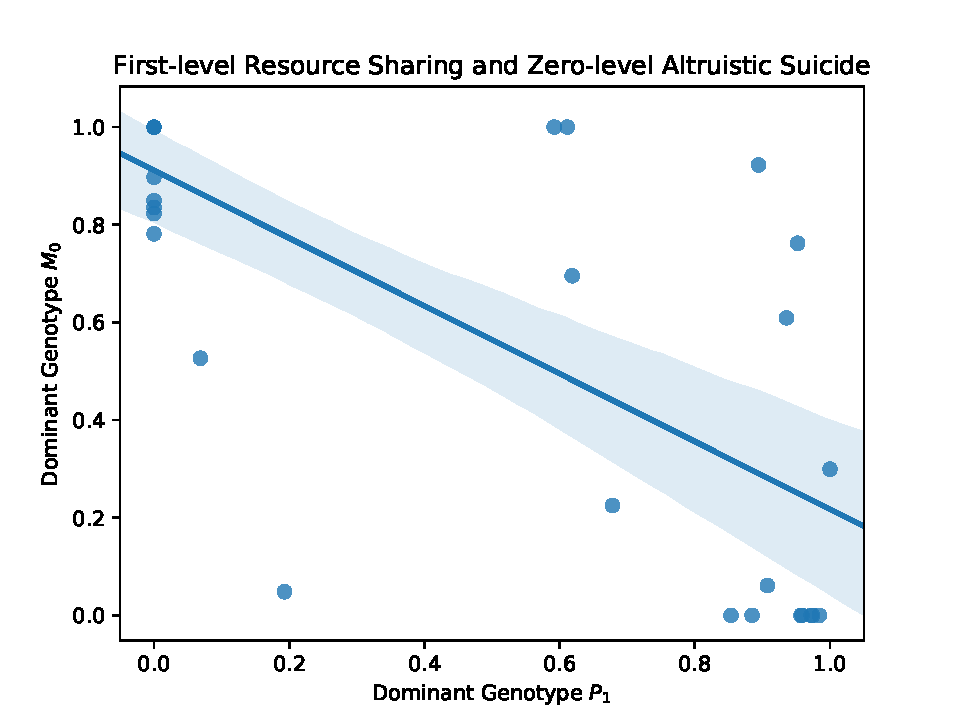
\includegraphics[width=\columnwidth]{img/champion_res_pool1_vs_champion_damage_suicide0}
  \caption{
  Correlation plot of dominant genotype $P_1$ and dominant genotype $M_{c}$.
  }
  \label{fig:champion_res_pool1_vs_champion_damage_suicide0}
\end{subfigure}%
~~
\begin{subfigure}[b]{\columnwidth}
  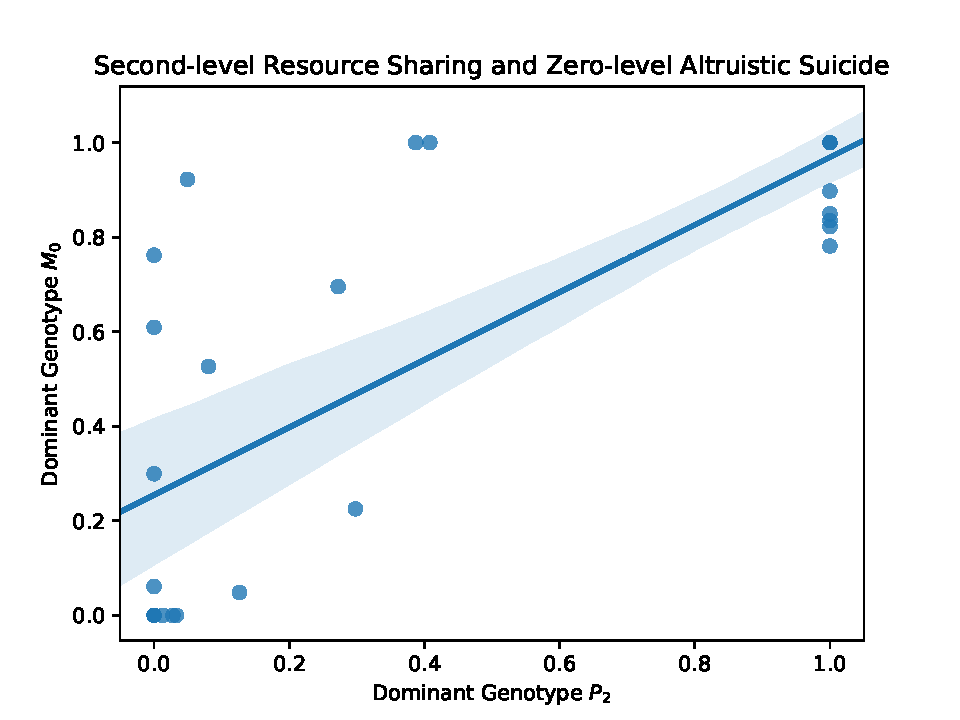
\includegraphics[width=\columnwidth]{img/champion_res_pool2_vs_champion_damage_suicide0}
  \caption{
  Correlation plot of dominant genotype $P_2$ and dominant genotype $M_{c}$.
  }
  \label{fig:champion_res_pool2_vs_champion_damage_suicide0}
\end{subfigure}

\caption{
Plots of dominant resource caching strategies and dominant apoptosis strategies.
A bootstrapped 95\% confidence interval for the fit is shaded.
Both correlations are statistically significant ($p < 0.05$; bootstrap test).
}
\label{fig:damage_suicide}
\end{center}
\end{figure*}
